\documentclass[12pt,letterpaper]{article}

\usepackage{amsmath, amsthm, amsfonts, amssymb}
\usepackage{microtype, parskip, graphicx}
\usepackage{multirow, morefloats, rotating}
\usepackage{caption, subcaption}
\usepackage{lineno}
\usepackage{afterpage}
\usepackage{hyperref}

\title{Report on Fossil/Not Fossil}


\begin{document}
\maketitle

\section{Set-Up}

We want to predict the expected diversity of a Macrostrat geological unit. We are focused on the diversity of individual biological classes. Geological units are described in terms of their lithological descriptions, areal extent, location, ``connectedness'' (units above/below), and other values. Lithological description is a compositional variable and thus has annoying properties which can prove difficult to interpret. 

The dataset is split into two sets: the late Ordovician (460.4--445.6) and the Hirnantian (445.6--443.8); the former is the training dataset while the latter is the testing dataset.


\section{Model}

The basics of the models used in this analysis is a hurdle model which is a mixture of a Bernoulli distribution and either a Poisson or Negative-Binomial distribution. The Bernoulli aspect describes the probability of observing 0 species in a geological unit, while the Poisson or Negative-Binomial describes the expected number of species present in that geological unit if there are more than 0.

Both parts of the mixture are modeled as regressions with all of the geological unit covariates as predictors.

The models are fit to the training dataset and the results of which are used to predict the diversity of the Hirnantian geological units. The approximate expected out-of-sample predictions were evaluated through 5 rounds of 5-fold cross-validation.

The models are fit in a fully Bayesian context using the Stan probabilistic programming language. Model fit for the complete training dataset is evaluated through a series of posterior predictive checks. Additionally, models are compared using WAIC and LOOIC which are estimates of comparative out-of-sample predictive performance.


\section{Results}

\subsection{Full data posterior predictive checks}
figures \ref{fig:ppc_mean}, \ref{fig:ppc_sd}, \ref{fig:ppc_ecdf}, \ref{fig:ppc_root}, \ref{fig:ppc_avgerr}.

\afterpage{\clearpage}
\begin{figure}[h]
  \centering
  
\includegraphics[width=\textwidth,height=0.8\textheight,keepaspectratio=true]{figure/ppc_mean}
  \caption{Mean of unit diversity. Distribution is estimated from posterior, vertical line is observed. Columns are by model type, rows are by taxonomic group.}
  \label{fig:ppc_mean}
\end{figure}

\afterpage{\clearpage}
\begin{figure}[h]
  \centering
  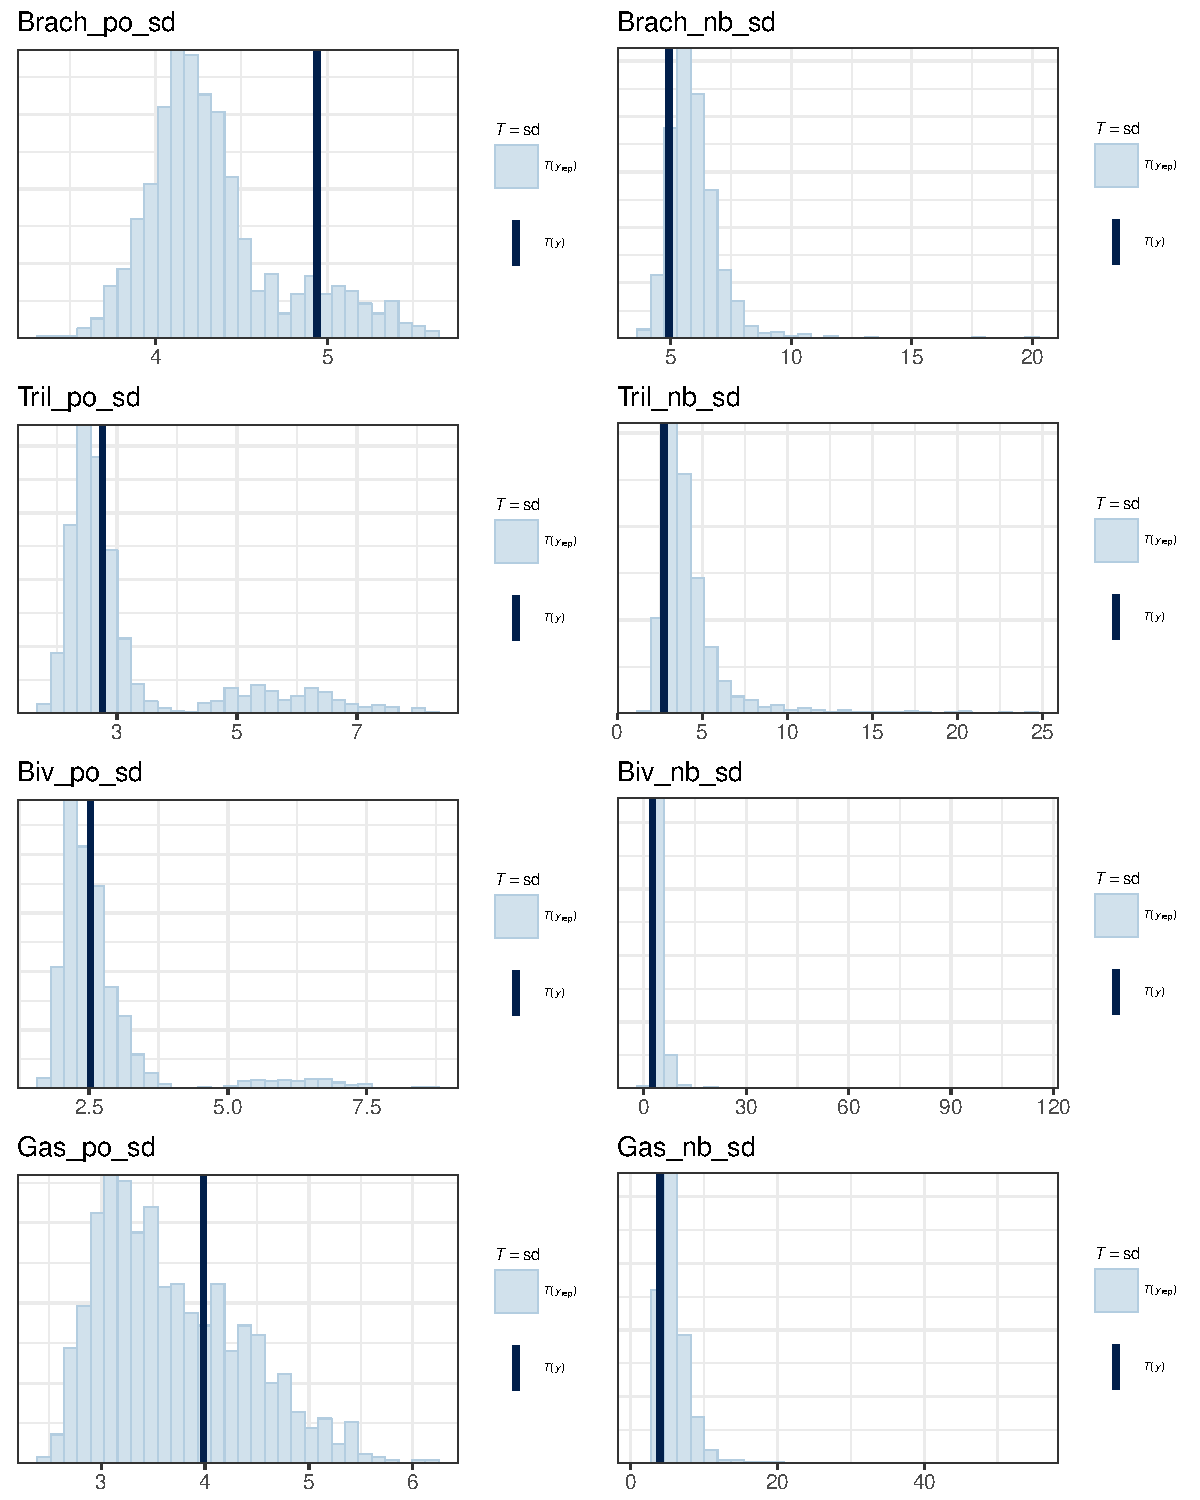
\includegraphics[width=\textwidth,height=0.8\textheight,keepaspectratio=true]{figure/ppc_sd}
  \caption{Standard deviation of unit diversity. Distribution is estimated from posterior, vertical line is observed. Columns are by model type, rows are by taxonomic group.}
  \label{fig:ppc_sd}
\end{figure}

\afterpage{\clearpage}
\begin{figure}[h]
  \centering
  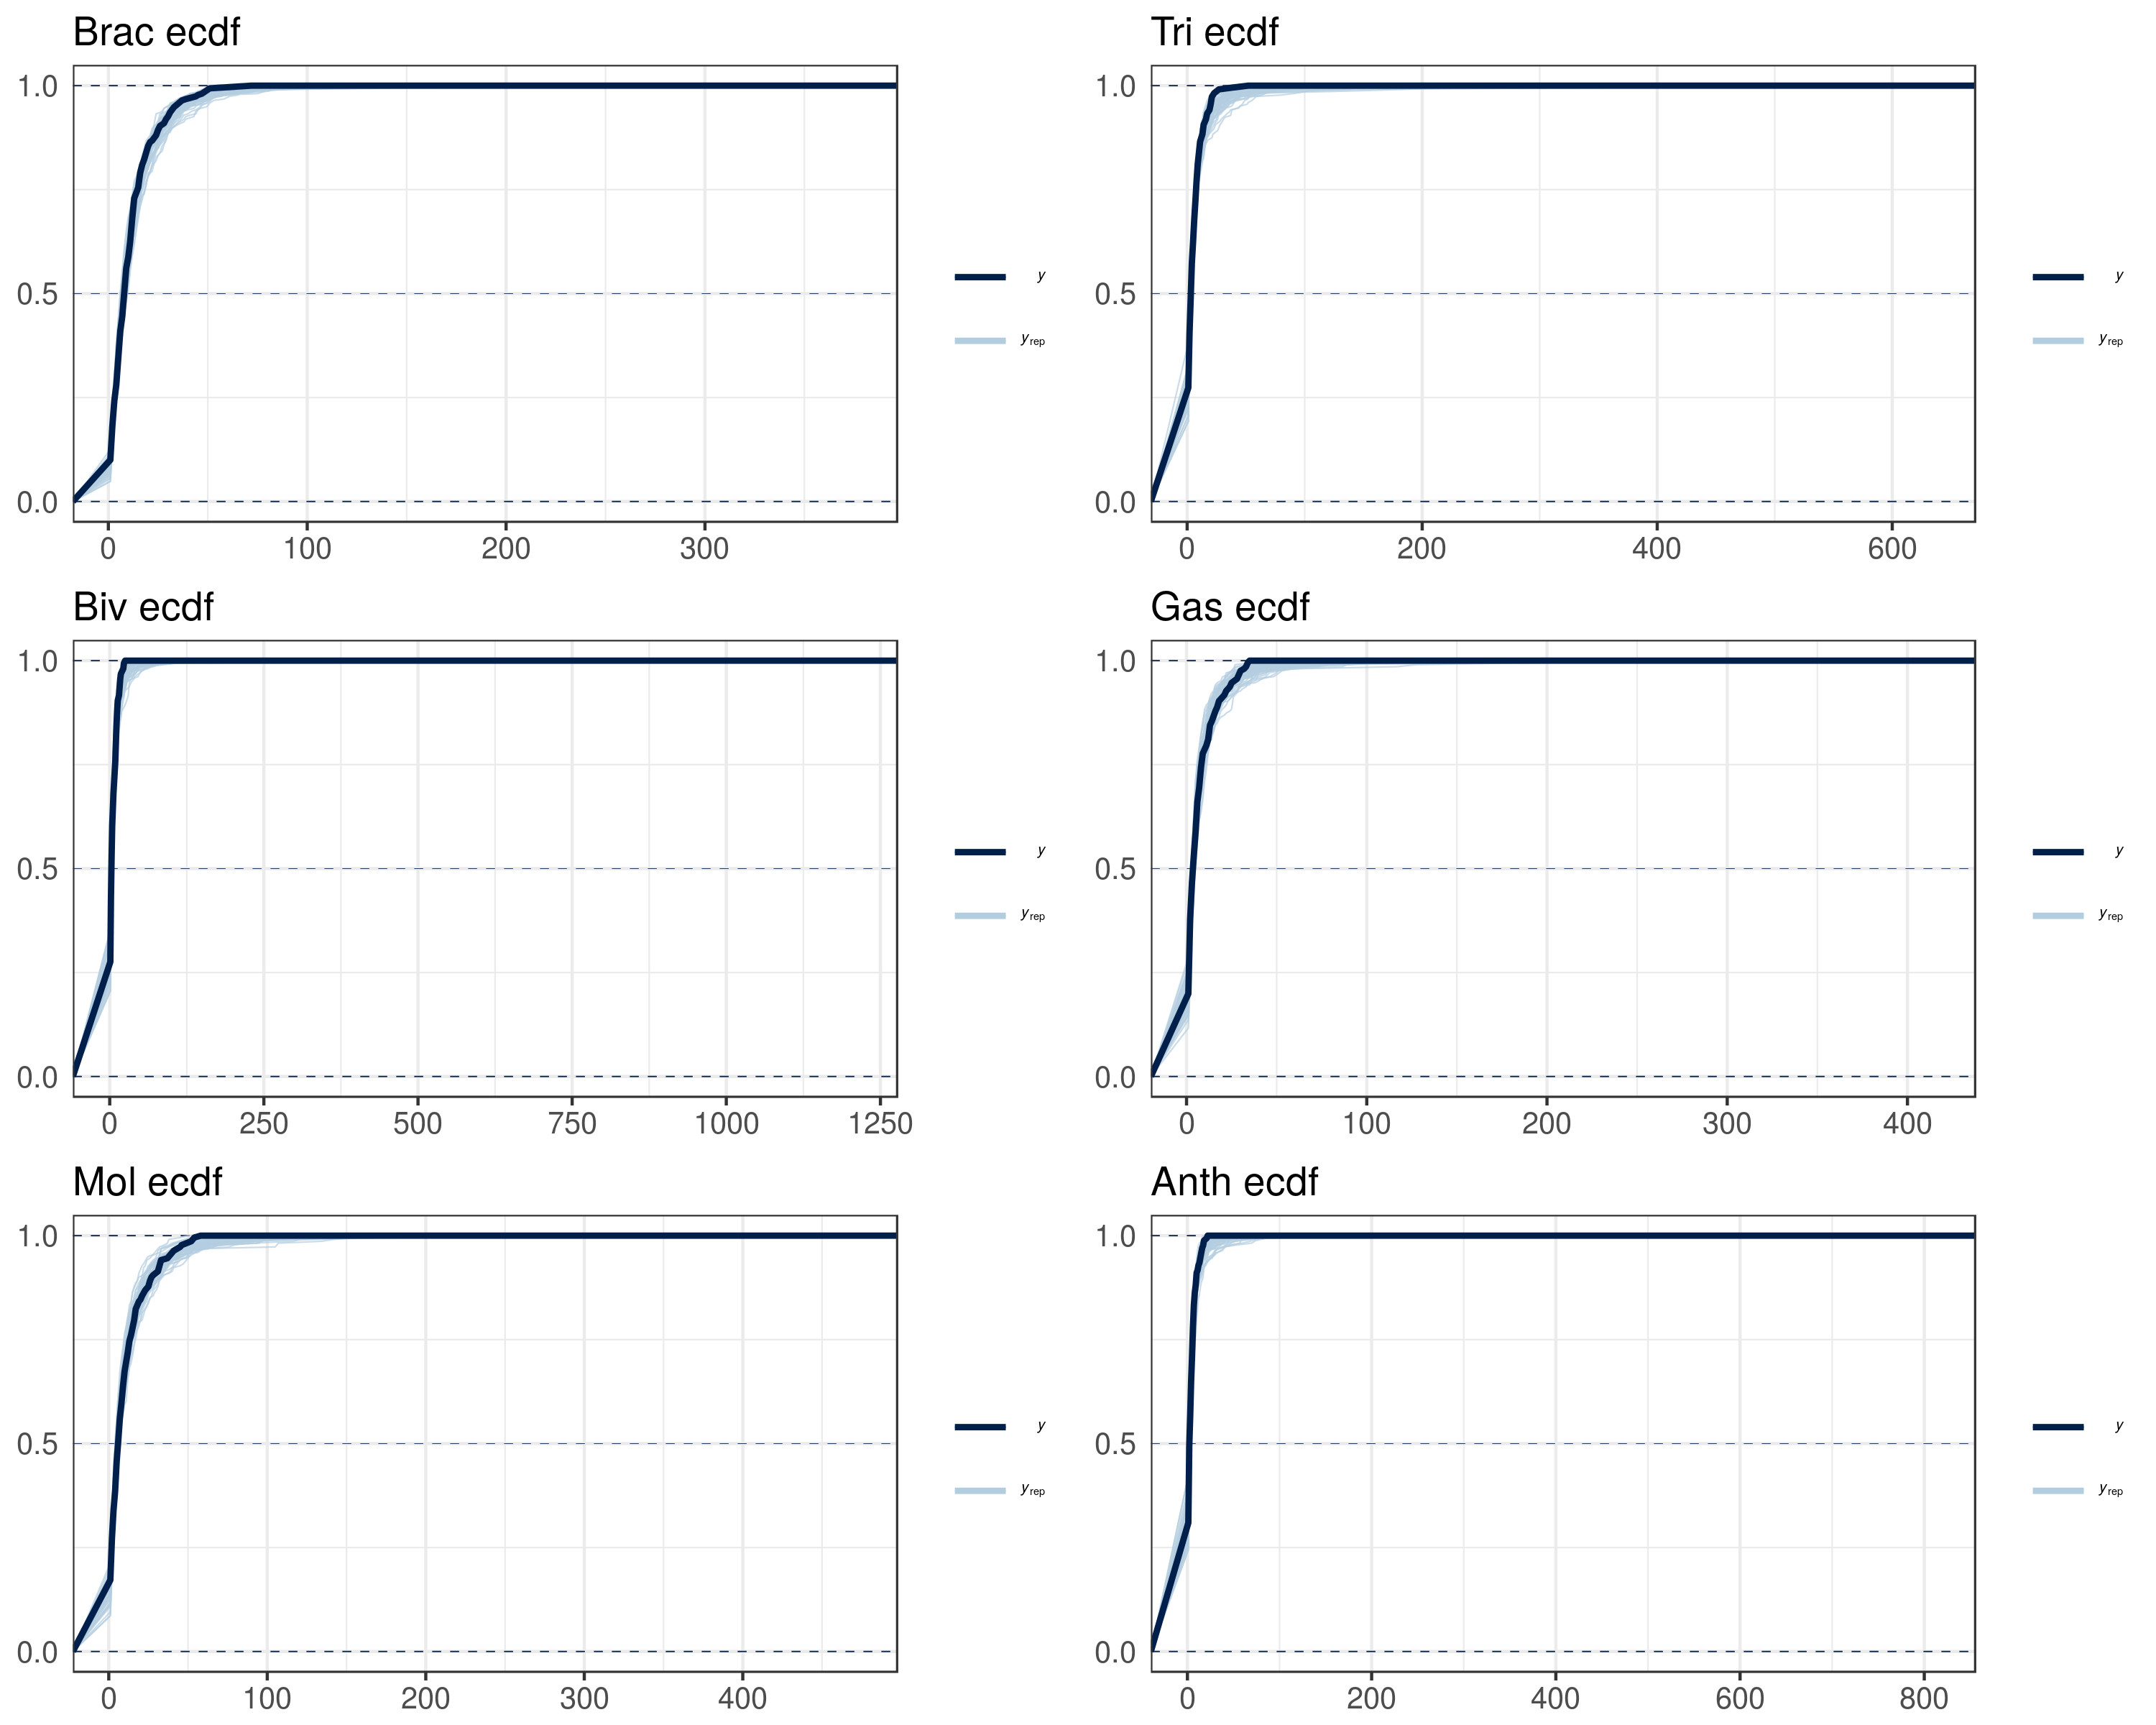
\includegraphics[width=\textwidth,height=0.8\textheight,keepaspectratio=true]{figure/ppc_ecdf}
  \caption{Empirical cumulative distribution function of unit diversity; that is, rank order proportional accumulation. Distribution is estimated from posterior, dark line is observed. Columns are by model type, rows are by taxonomic group.}
  \label{fig:ppc_ecdf}
\end{figure}

\afterpage{\clearpage}
\begin{figure}[h]
  \centering
  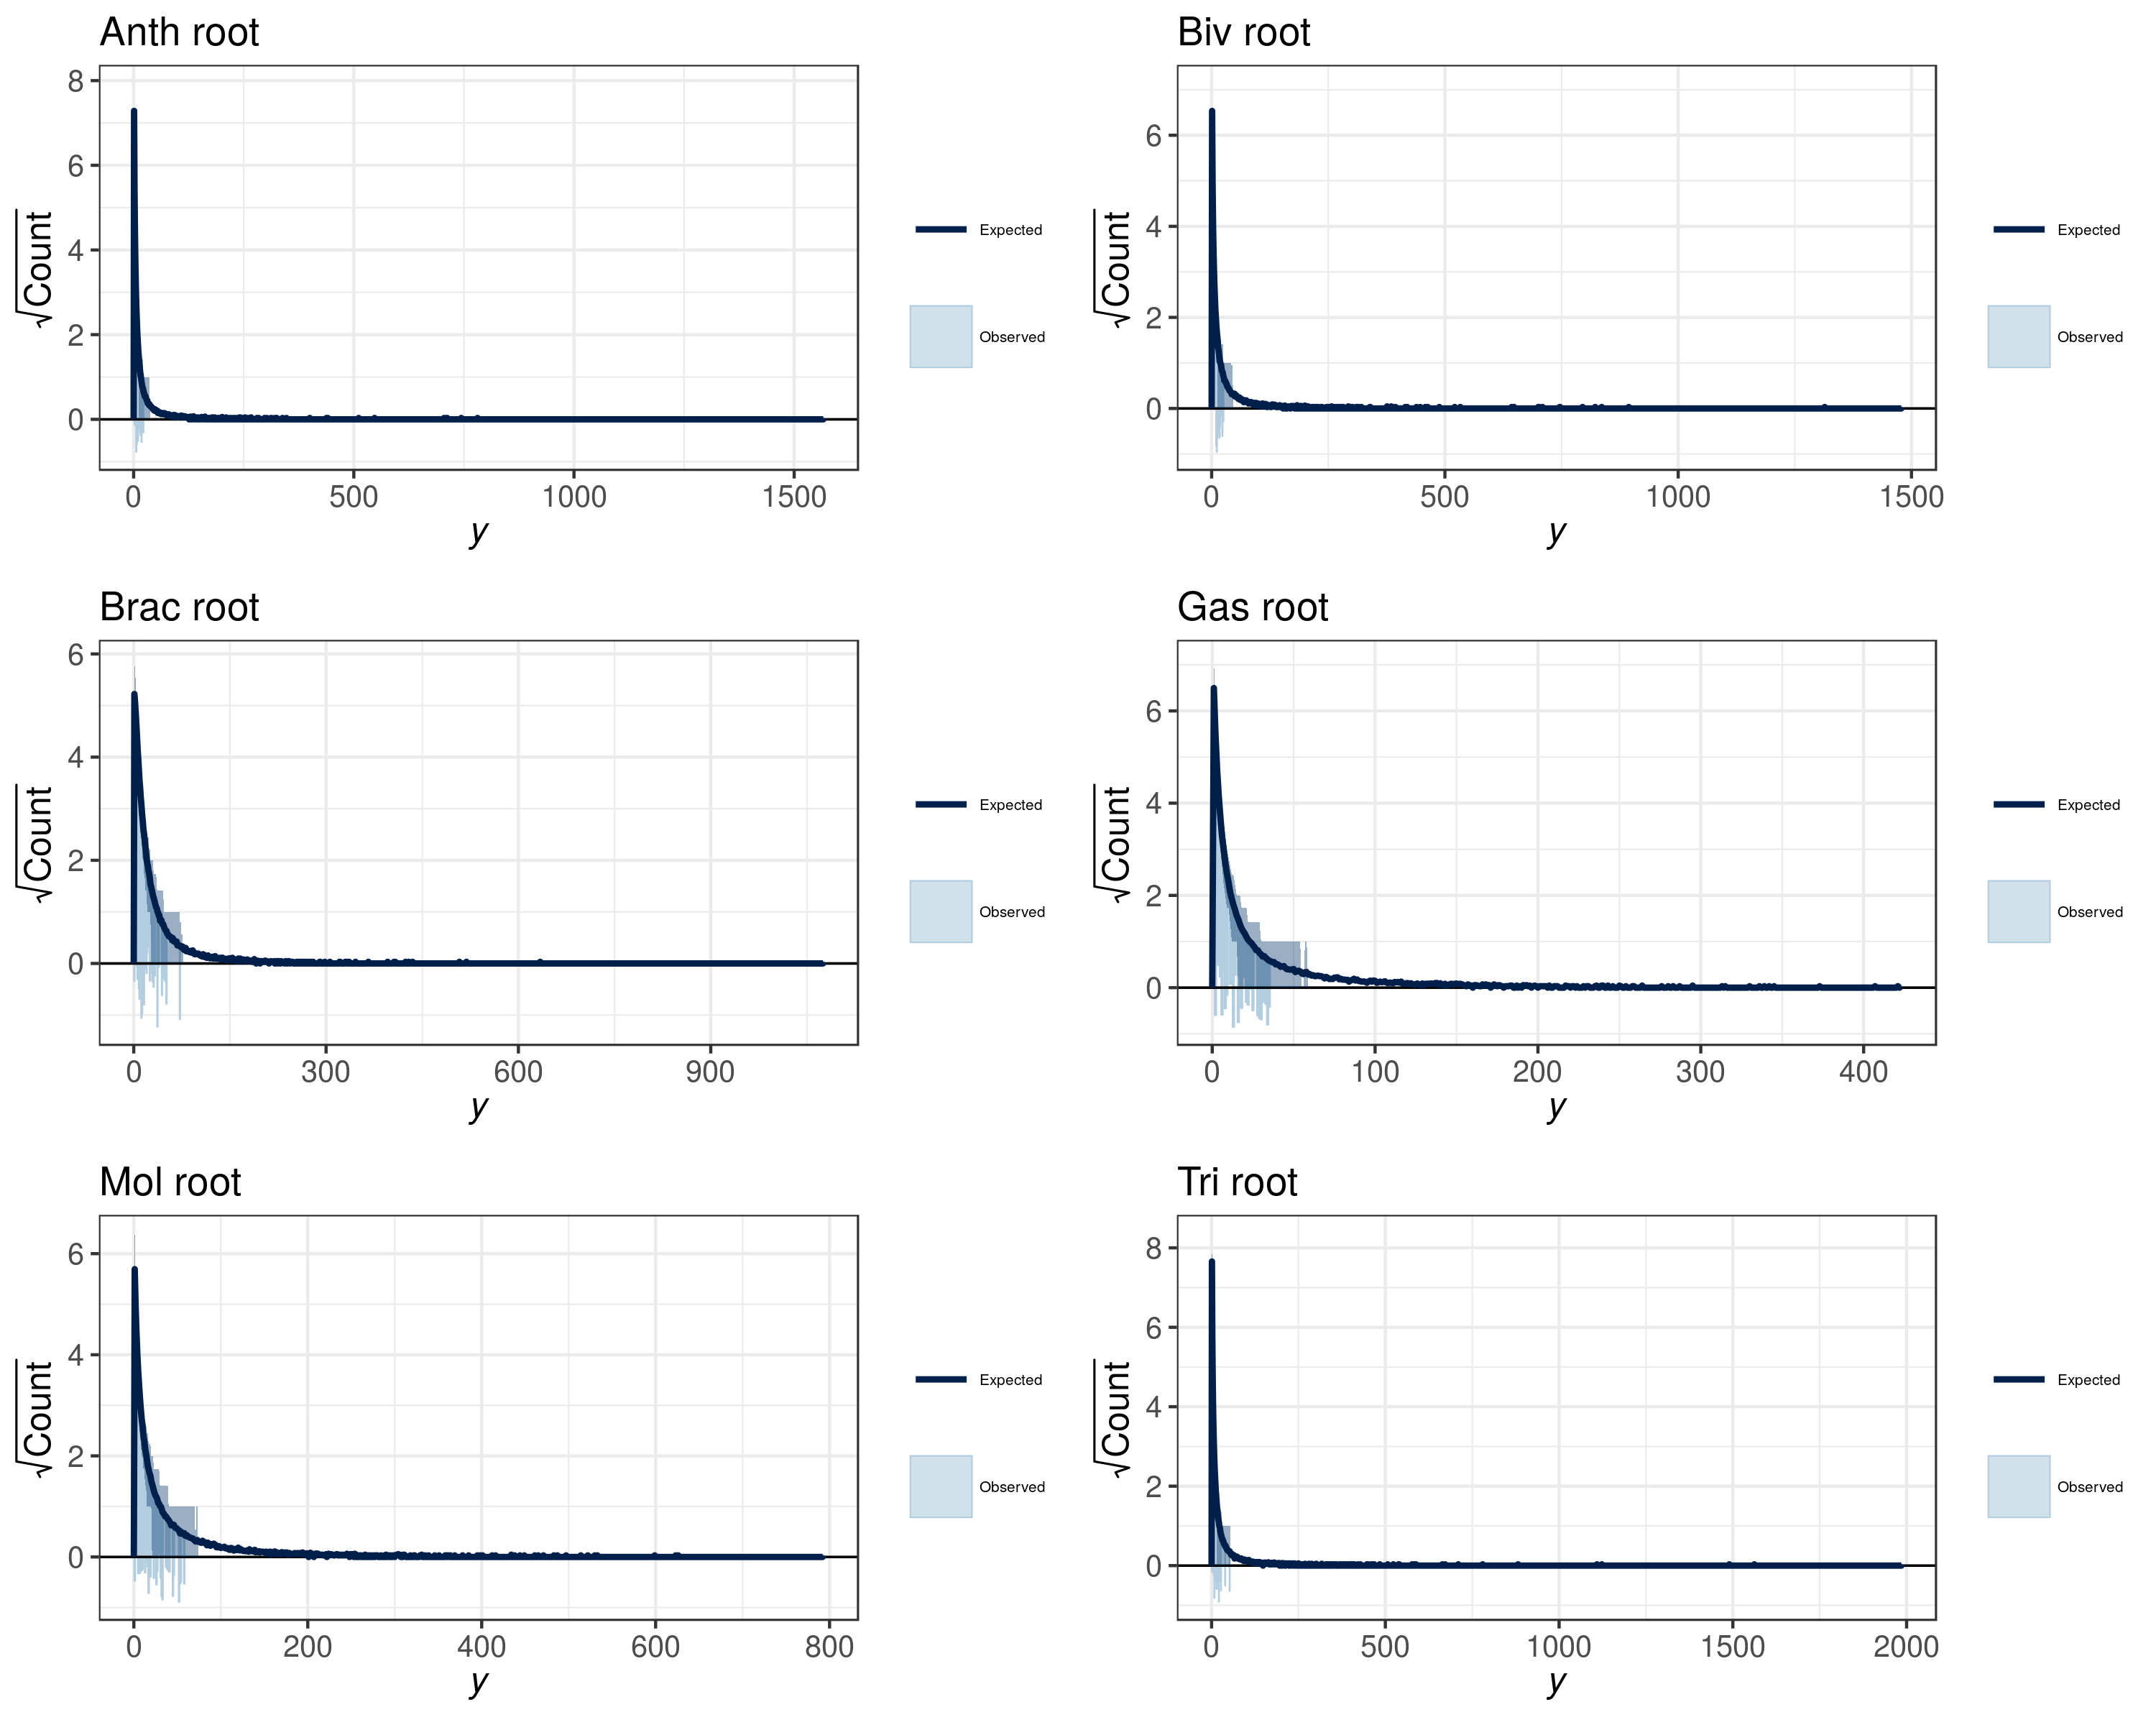
\includegraphics[width=\textwidth,height=0.8\textheight,keepaspectratio=true]{figure/ppc_root}
  \caption{Rootogram of unit diversity. Distribution is estimated from posterior, hanging histogram is is observed. If histogram is above x-axis, overestimate; if histogram is below x-axis, underestimate. Columns are by model type, rows are by taxonomic group.}
  \label{fig:ppc_root}
\end{figure}

\afterpage{\clearpage}
\begin{figure}[h]
  \centering
  
\includegraphics[width=\textwidth,height=0.8\textheight,keepaspectratio=true]{figure/ppc_avgerr}
  \caption{Average error of estimated unit diversity. Comparison is between observed diversity and estimated diversity. Columns are by model type, rows are by taxonomic group.}
  \label{fig:ppc_avgerr}
\end{figure}


\subsection{K-fold cross-validation results}
figures \ref{fig:cv_rmse}.

\afterpage{\clearpage}
\begin{figure}[h]
  \centering
  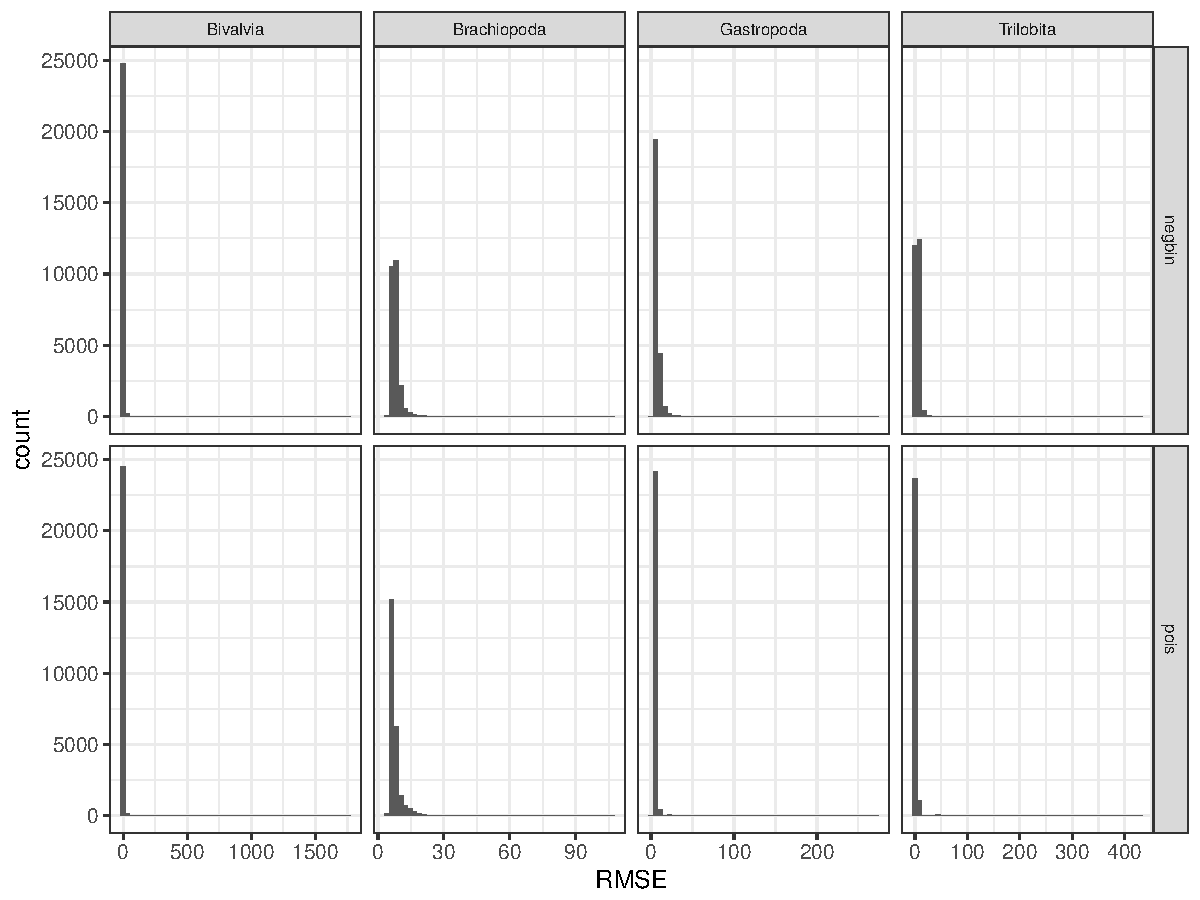
\includegraphics[width=\textwidth,height=0.8\textheight,keepaspectratio=true]{figure/cv_rmse}
  \caption{Posterior estimates of the expected out-of-sample error based on 5 rounds of 5-fold cross-validation. Columns are by model type, rows are by taxonomic group.}
  \label{fig:cv_rmse}
\end{figure}


\subsection{Regression coefficients}
figures \ref{fig:arth_coefs}, \ref{fig:brach_coefs}, \ref{fig:mol_coefs}.

\afterpage{\clearpage}
\begin{figure}[h]
  \centering
  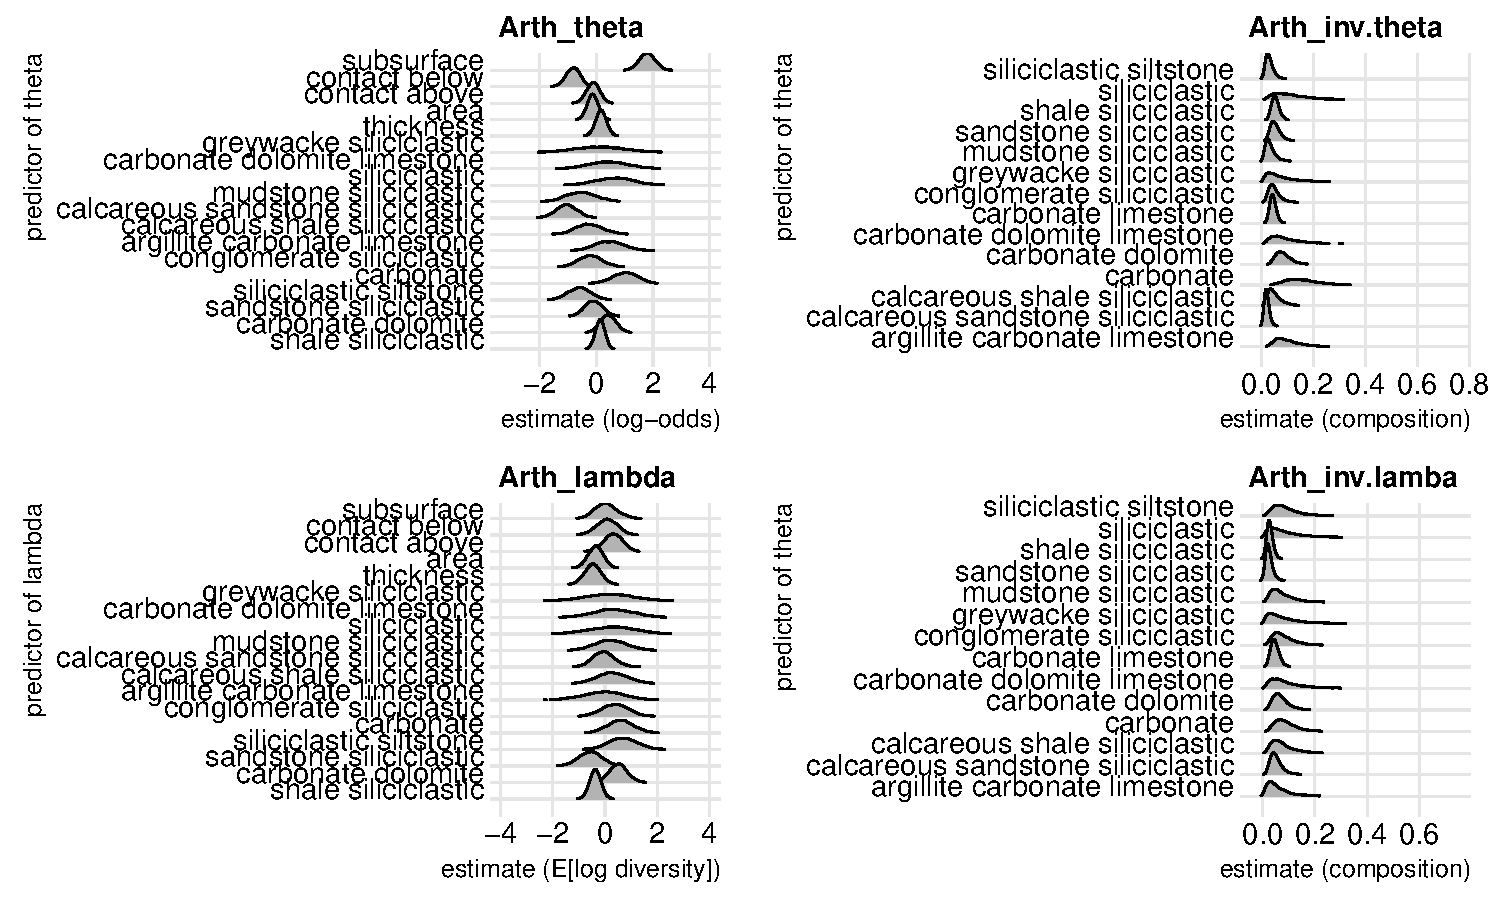
\includegraphics[width=\textwidth,height=0.8\textheight,keepaspectratio=true]{figure/arth_coefs}
  \caption{left: coefficients from the arthropod analysis. right: regression coefs for compositional variables back-transformed into composition units. theta is for binomial part (i.e. zeroes), lambda is for poisson or negative binomial part (i.e. non-zeroes)}
  \label{fig:arth_coefs}
\end{figure}

\afterpage{\clearpage}
\begin{figure}[h]
  \centering
  
\includegraphics[width=\textwidth,height=0.8\textheight,keepaspectratio=true]{figure/brach_coefs}
  \caption{left: coefficients from the brachiopod analysis. right: regression coefs for compositional variables back-transformed into composition units. theta is for binomial part (i.e. zeroes), lambda is for poisson or negative binomial part (i.e. non-zeroes)}
  \label{fig:brach_coefs}
\end{figure}

\afterpage{\clearpage}
\begin{figure}[h]
  \centering
  
\includegraphics[width=\textwidth,height=0.8\textheight,keepaspectratio=true]{figure/mol_coefs}
  \caption{left: coefficients from the mollusc analysis. right: regression coefs for compositional variables back-transformed into composition units. theta is for binomial part (i.e. zeroes), lambda is for poisson or negative binomial part (i.e. non-zeroes)}
  \label{fig:mol_coefs}
\end{figure}


\subsection{Predictive results}
figures \ref{fig:pred_mean}, \ref{fig:pred_sd}, \ref{fig:pred_ecdf}, \ref{fig:pred_root}, \ref{fig:pred_avgerr}.

\afterpage{\clearpage}
\begin{figure}[h]
  \centering
  
\includegraphics[width=\textwidth,height=0.8\textheight,keepaspectratio=true]{figure/pred_mean}
  \caption{Mean of unit diversity for testing dataset. Distribution is estimated from posterior, vertical line is observed. Columns are by model type, rows are by taxonomic group.}
  \label{fig:pred_mean}
\end{figure}

\begin{figure}[h]
\afterpage{\clearpage}
  \centering
  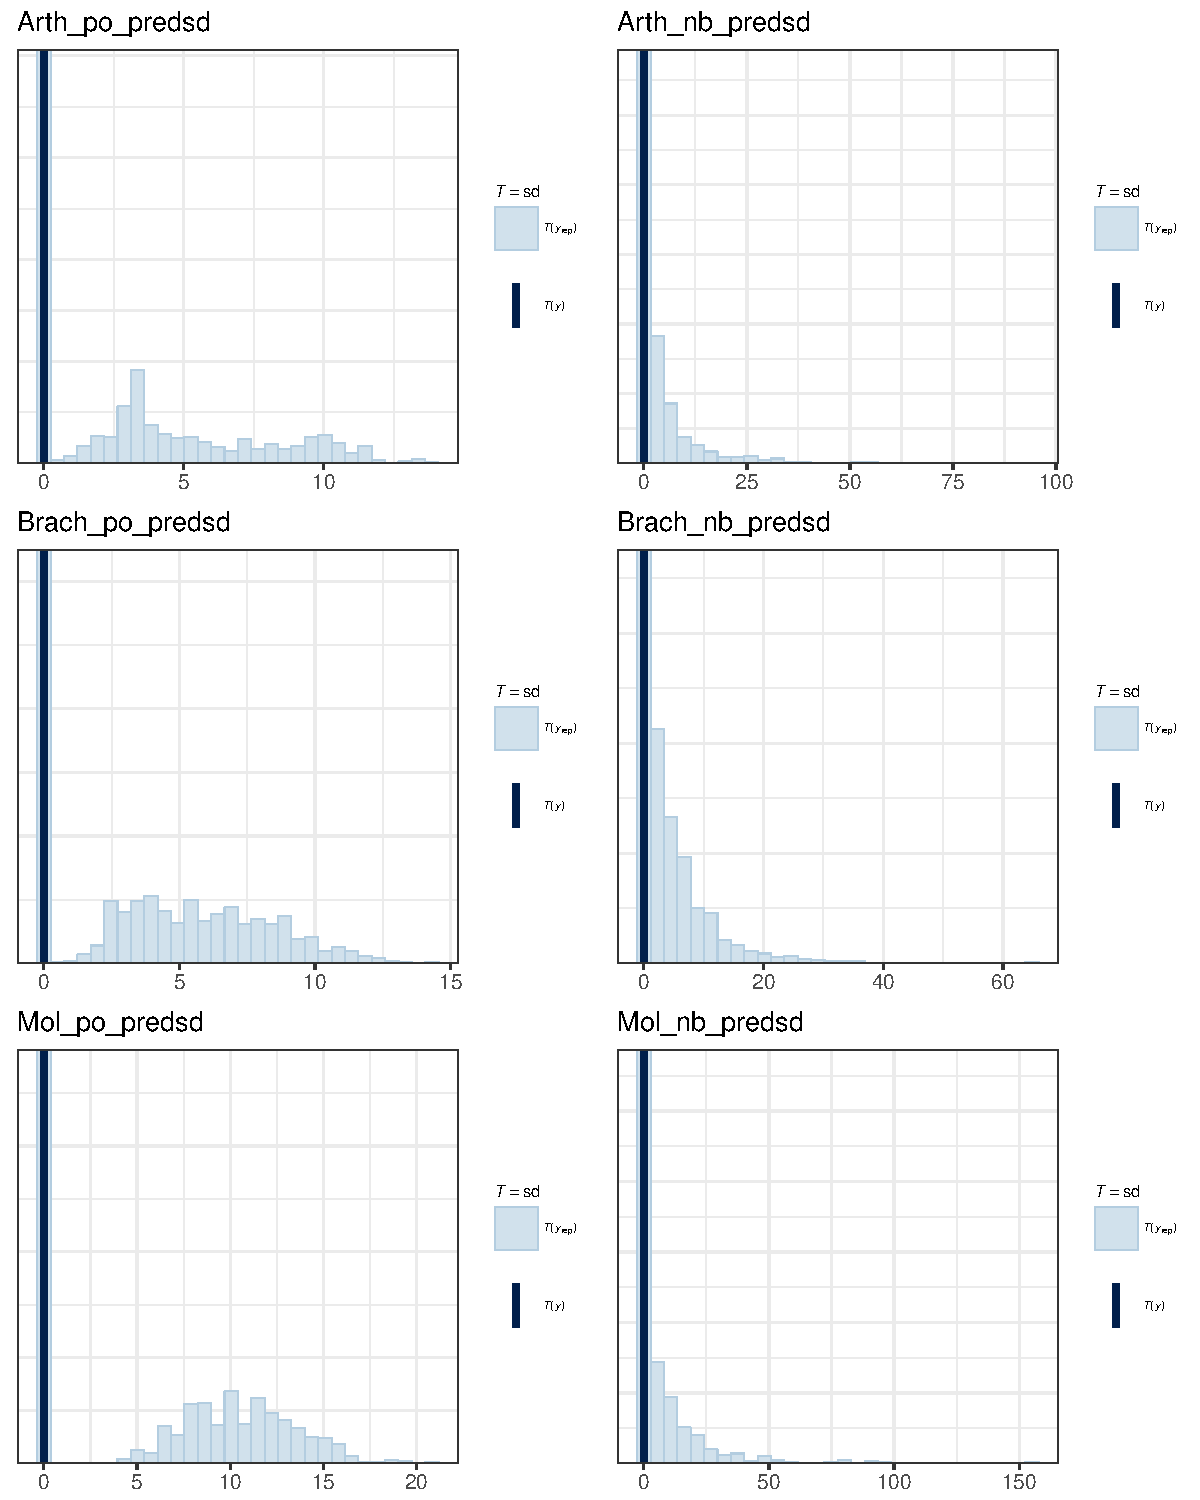
\includegraphics[width=\textwidth,height=0.8\textheight,keepaspectratio=true]{figure/pred_sd}
  \caption{Standard deviation of unit diversity for testing dataset. Distribution is estimated from posterior, vertical line is observed. Columns are by model type, rows are by taxonomic group.}
  \label{fig:pred_sd}
\end{figure}

\afterpage{\clearpage}
\begin{figure}[h]
  \centering
  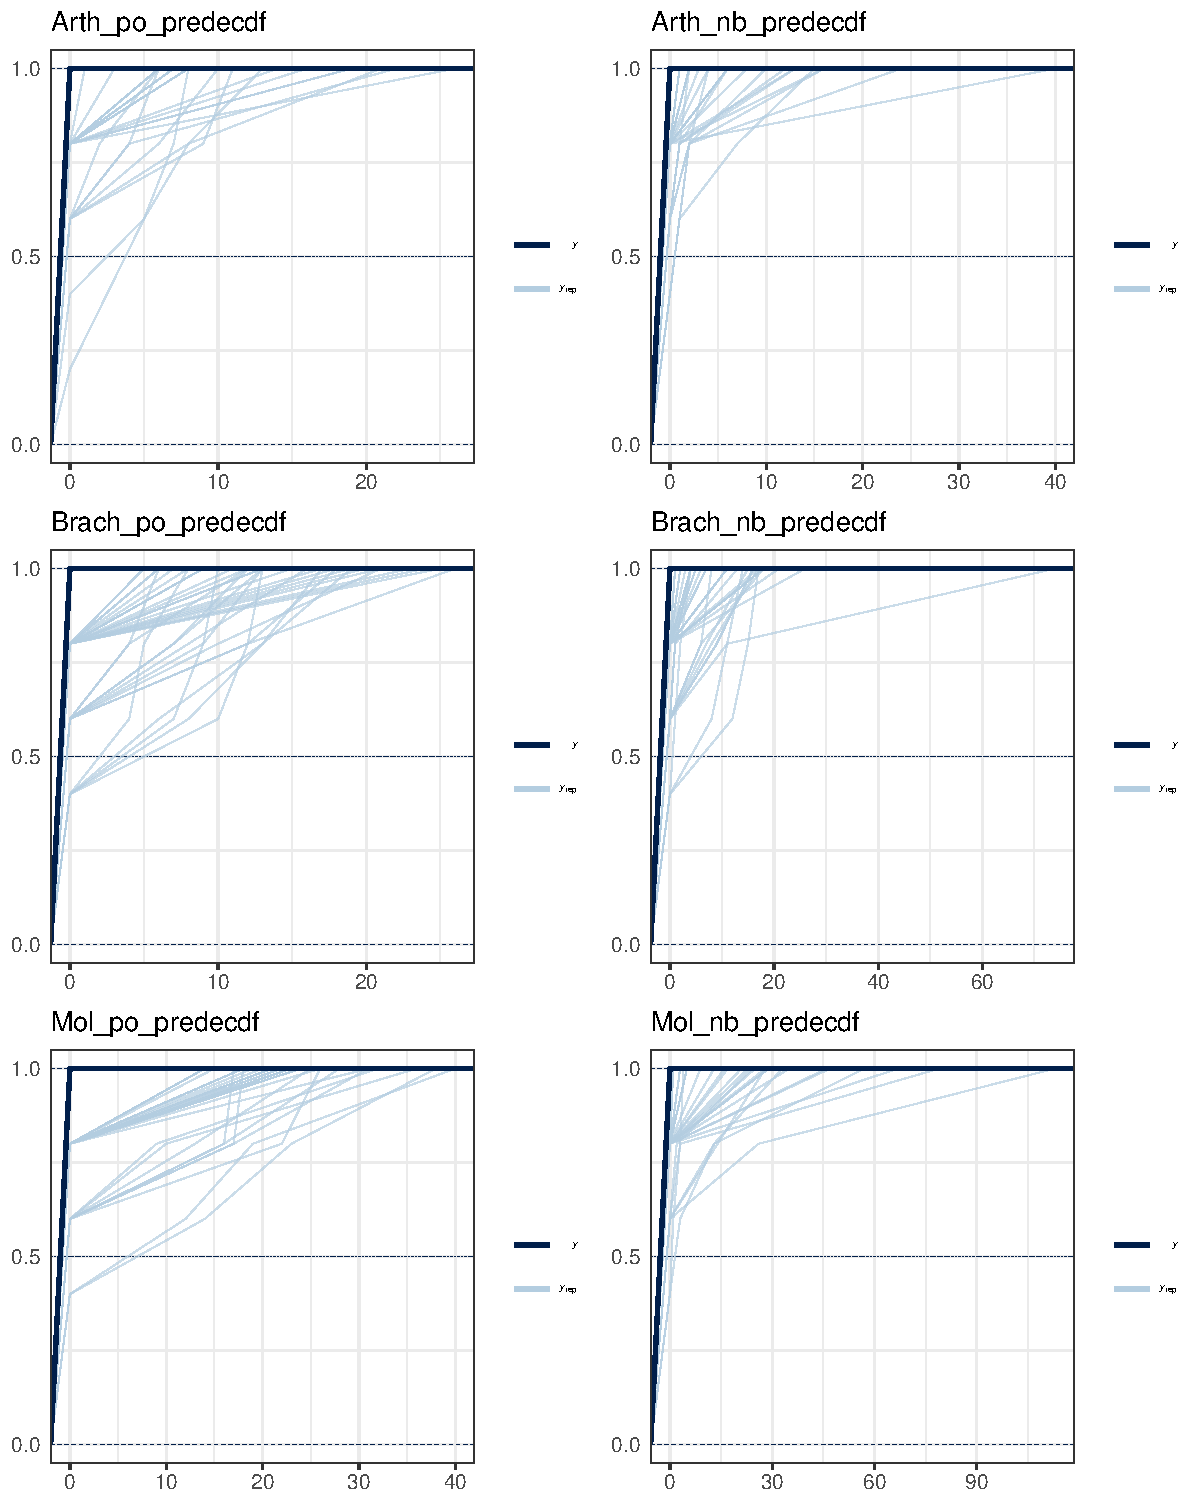
\includegraphics[width=\textwidth,height=0.8\textheight,keepaspectratio=true]{figure/pred_ecdf}
  \caption{Empirical cumulative distribution function of unit diversity for testing dataset; that is, rank order proportional accumulation. Distribution is estimated from posterior, dark line is observed. Columns are by model type, rows are by taxonomic group.}
  \label{fig:pred_ecdf}
\end{figure}

\afterpage{\clearpage}
\begin{figure}[h]
  \centering
  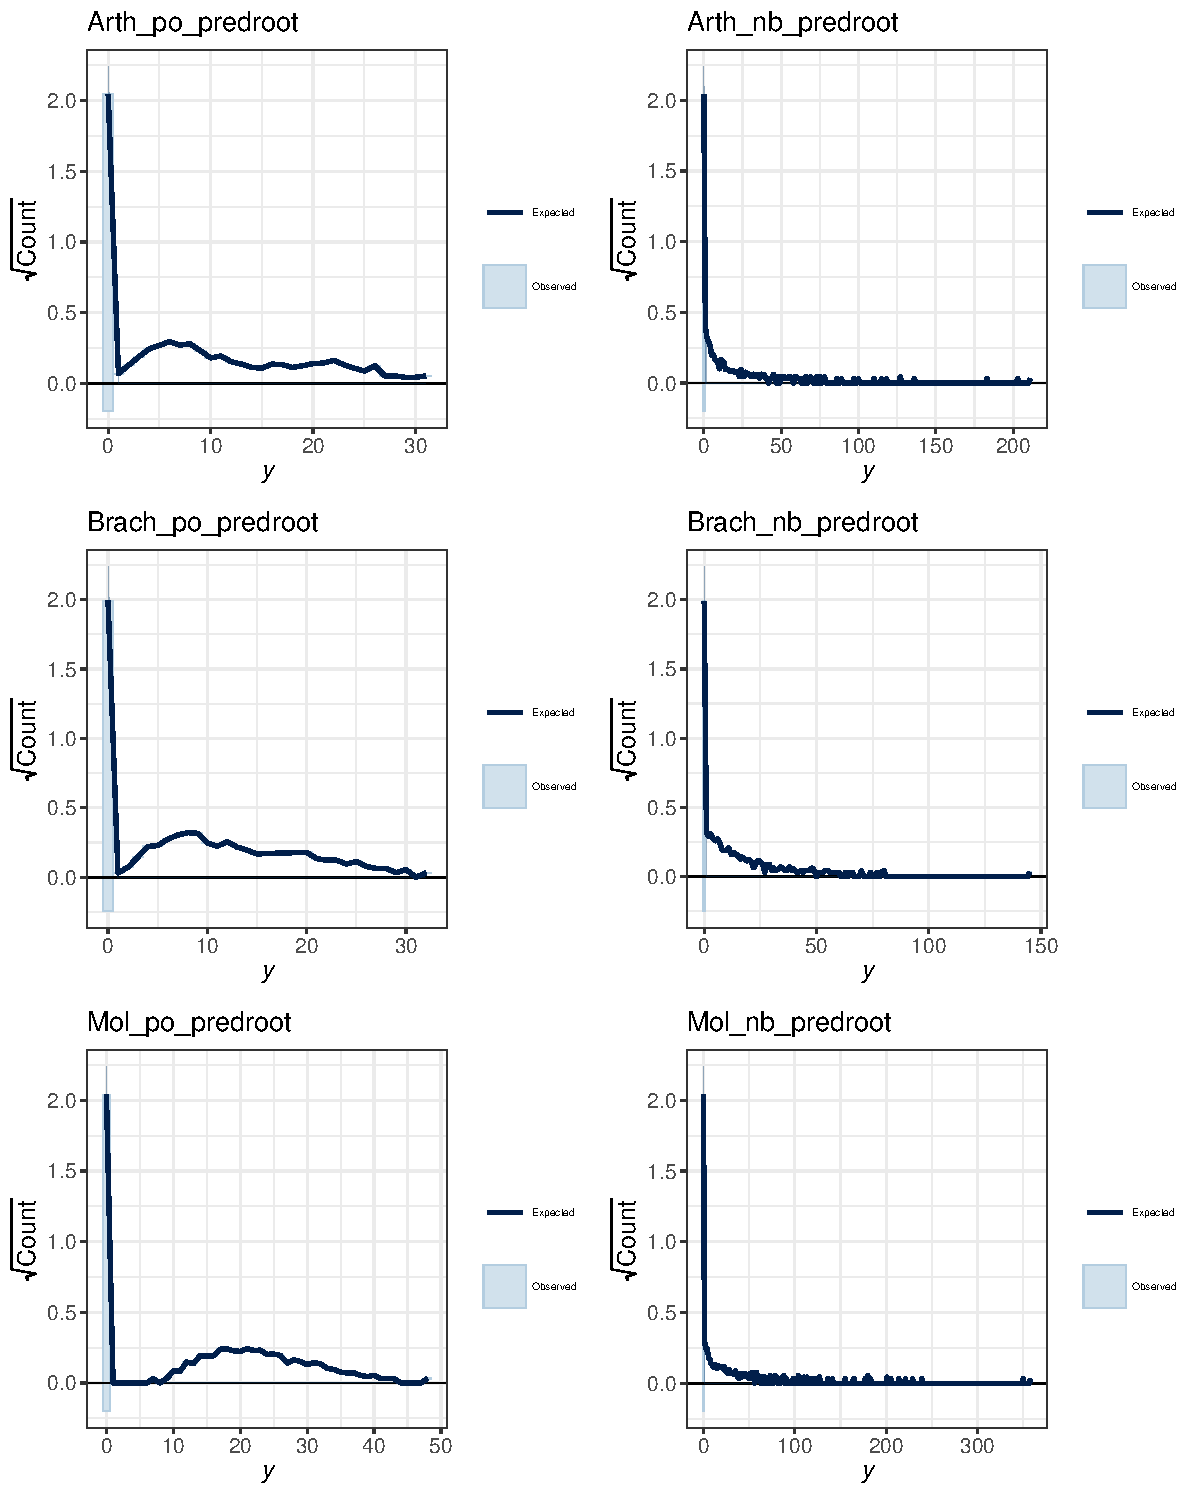
\includegraphics[width=\textwidth,height=0.8\textheight,keepaspectratio=true]{figure/pred_root}
  \caption{Rootogram of unit diversity for testing dataset. Distribution is estimated from posterior, hanging histogram is is observed. If histogram is above x-axis, overestimate; if histogram is below x-axis, underestimate. Columns are by model type, rows are by taxonomic group.}
  \label{fig:pred_root}
\end{figure}

\afterpage{\clearpage}
\begin{figure}[h]
  \centering
  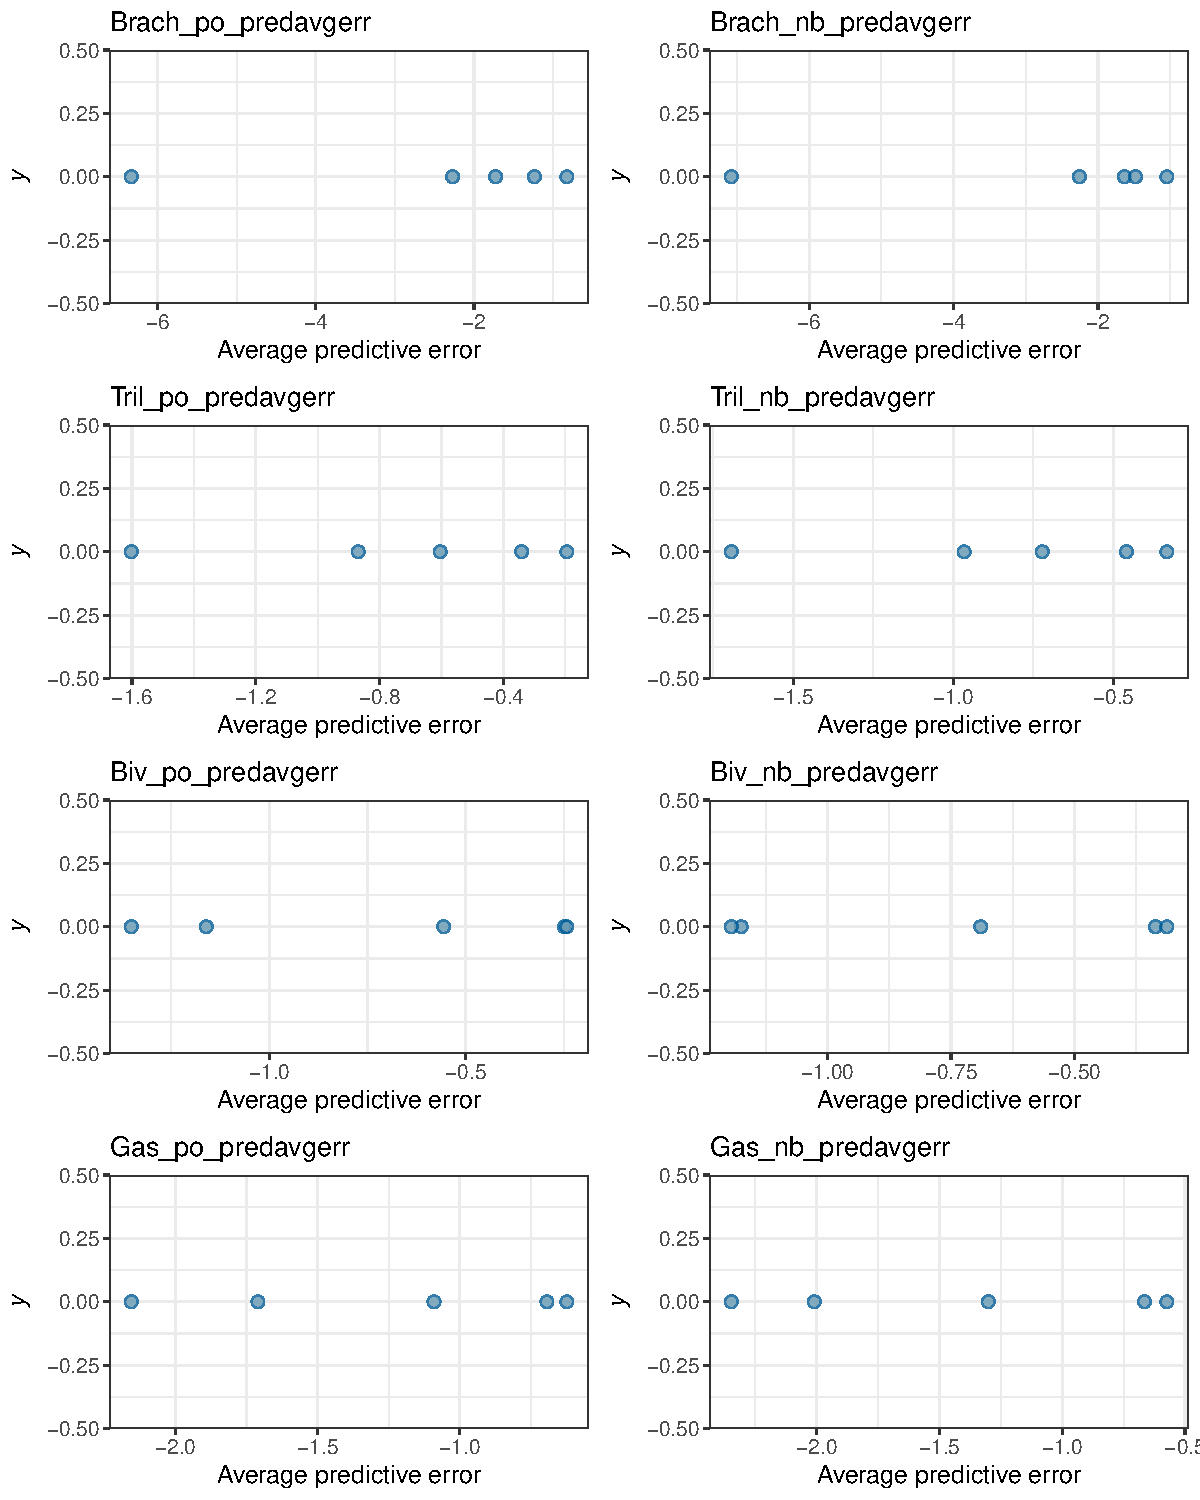
\includegraphics[width=\textwidth,height=0.8\textheight,keepaspectratio=true]{figure/pred_avgerr}
  \caption{Average error of estimated unit diversity for testing dataset. Comparison is between observed diversity and estimated diversity. Columns are by model type, rows are by taxonomic group.}
  \label{fig:pred_avgerr}
\end{figure}


\end{document}
